%!TEX root = ../thesis.tex
%*******************************************************************************
%****************************** Second Chapter *********************************
%*******************************************************************************

\chapter{Encoding Locations}

\ifpdf
  \graphicspath{{Chapter2/Figs/Raster/}{Chapter2/Figs/PDF/}{Chapter2/Figs/}}
\else
  \graphicspath{{Chapter2/Figs/Vector/}{Chapter2/Figs/}}
\fi

\section{Introduction}
% Waar gaat dit hoofdstuk over?
To answer in what way locations can be represented to be universally interpretable, the definition of a location must be well understood. Encoding of locations has historically been of great importance, and is always being modernized. This chapter aims to find the best method of representing locations that is universally interpretable and most importantly usable in this project. GPS and Postal Codes are globally adopted and have proven to be reliable methods of encoding locations. Locations, plurally, suggesting that more than one location should be encoded. This is where the challenge lies.

\section{A Brief History Of Geographic Locations}

A location is roughly described as a place or position. Throughout history, various navigational techniques and tools like the sextant, nautical chart and marinner's compass were used, measuring the altitude of the North Star to determine the latitude $\phi$, in conjunction with a chronometer to determine the longitude $\lambda$ of a location on the Earth's surface.

\begin{figure}[htbp!]
  \centering
  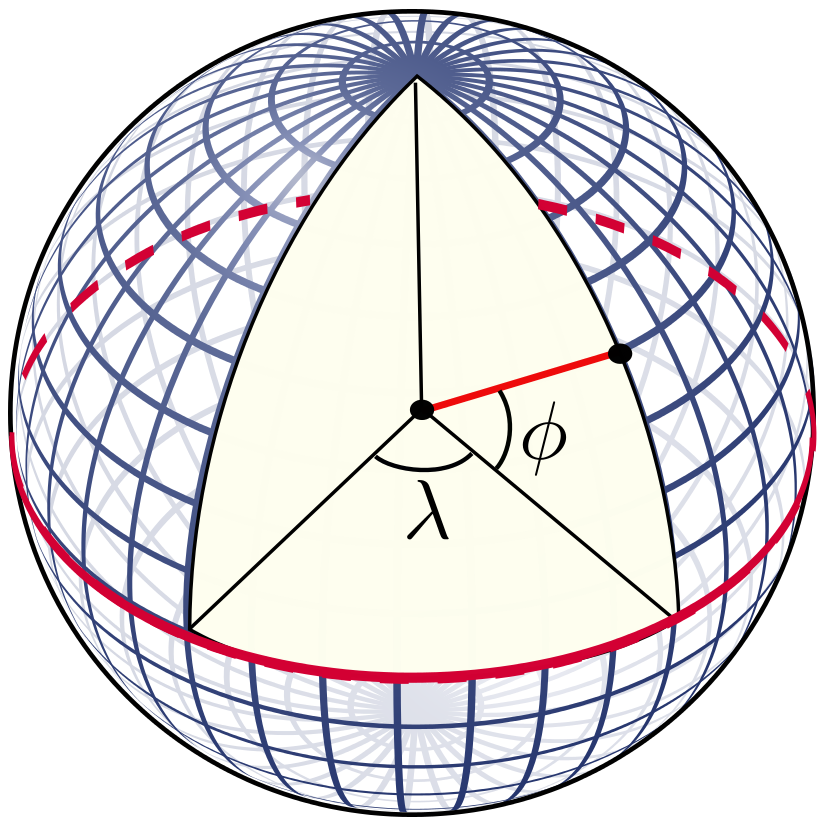
\includegraphics[width=.2\textwidth]{LatLngSphere}
  \caption[LatLngSphere]{A perspective view of the Earth showing how latitude and longitude are defined on a spherical model.}
  \label{fig:latlngsphere}
\end{figure}

Modern navigation relies on sattelites that are capable of providing information to determine a location with an accuracy of 9 meters. The precision of hybrid methods using cell towers and Wi-Fi Location Services enables precise tracking of modern devices. Latitude and longitude are often referred to as GPS coordinates, as GPS is often used to calculate latitude and longitude by receiving position and time code sequences from at least four sattelites. Addresses are another representation of a location used in navigation. Addresses are easier to communicate than a pair of GPS coordinates, but can be ambiguous, imprecise, inconsistent in format. Addresses commonly make use of Postal Code systems, which have reliably been assigned to geographical areas with the purpose of sorting mail. Although even today, there are countries that do not have a Postal Code system.
A location being roughly described as a place or position, can be decomposed as an abstract term to describe physical or imaginary areas with varying radiusses and shapes. You could prepend 'the location of' to the following terms as an example: America, the birthplace of Sokrates, Wall Street, the center of the universe, the Laryngeal Nerve of the Giraffe, churches in the Netherlands. The final example presents the main challenge of this project.

\section{Useful Location Types}

While setting up a backlog, a shared knowledge about the terminology used in the issues must be achieved. In the pregame document, the term "area" was defined as a collection of three or more coordinate pairs, or a collection of postal codes. A "point" was defined as one distinct coordinate pair or one distinct postal code. This way a location could either be an area or a point, with which all possibilities are covered. As stated in appendix \mynote{appendix pregame ref} definition of an area is precise, unambiguous and easy to use in compare in computer programs. A single point may match another single point if it’s the exact same point. A point may be sitting on top of a line or is contained within an area. The only other option is the negation of these statements. Because use cases for lines will be non-existent, points and areas are the proper candidates for spatial queries.

\section{Requisites of Locations}

A taxi company director wants to be able to set price or define discounts from or to a certain location. They would like to define prices based only on departure locations, or only on destination locations, or both. For example: 'to Schiphol, a trip should cost \euro 10,-', or 'from Falke hotels a trip should cost \euro 5,-', or 'from Falke hotels to Schiphol, the km price should be \euro 0,60'. In the current implementation, a record would be stored containing departure location, destination location and price for every combination, where locations were defined as zip codes. Instead, it would make sense to be able to reuse locations after they have been defined once.

\section{Literature Review}



In what way can locations be represented to be universally interpretable?
\begin{enumerate}
  \item Which types of locations should be distinguished?
  \item What are the main differences between postal systems used around the globe?
  \item Can postal codes be abstracted to geospatial data while retaining the same usefulness in the system?
  \item How can different types of locations be effectively stored in a database?
\end{enumerate}
